\documentclass[11pt]{article}
\usepackage{amssymb}
\usepackage{amsmath}
\usepackage{amsthm}
%\usepackage{fullpage}
\usepackage{comment}
\usepackage{hyperref}
\usepackage{graphicx}
\usepackage{clrscode3e}
\usepackage[font=scriptsize]{caption}
\usepackage{fancyhdr}
\usepackage[margin=1in]{geometry}
\usepackage{enumitem}
\usepackage{tikz}
\usepackage{enumitem}
\usetikzlibrary{shapes}

\includecomment{solution}
\includecomment{question}
\setlength{\parskip}{1ex}
\def\nats {{\mathbb N}}
\def\ints {{\mathbb Z}}
\def\R {{\mathbb R}}
\DeclareMathOperator*{\Argmin}{argmin}
\DeclareMathOperator*{\Argmax}{argmax}
\newcommand{\Implies}{\mbox{ IMPLIES }}
\newcommand{\Or}{\mbox{ OR }}
\renewcommand{\And}{\mbox{ AND }}
\newcommand{\Not}{\mbox{NOT }}
\newcommand{\Iff}{\mbox{ IFF }}
\newcommand{\True}{\mbox{True}}
\newcommand{\False}{\mbox{False}}

\newcommand{\Exp}{\mathbb{E}}
\newcommand{\Var}{\mathrm{Var}}

\newcommand{\cvec}[2]{\big[\begin{smallmatrix} #1 \\ #2 \end{smallmatrix}\big]}
\newcommand{\Cvec}[2]{\begin{bmatrix} #1 \\ #2 \end{bmatrix}}

\newcommand*{\Scale}[2][4]{\scalebox{#1}{$#2$}}
\newcommand*{\Resize}[2]{\resizebox{#1}{!}{$#2$}}

\newtheorem{theorem}{Theorem}
\newtheorem{lemma}{Lemma}
\newtheorem{corollary}[lemma]{Corollary}

\pagestyle{fancy}
\fancyhf{}
\rhead{Assignment 3}
\chead{Kevin Gao (1006967338)}
\lhead{CSC 2420}
\cfoot{\thepage}

\begin{document}

\section*{Assignment 3}

\begin{enumerate}[leftmargin=16pt]
    \item Consider $n \times n$ matrices with entries from some infinite ring $\R$ (e.g., the integers). Someone claims to have an algorithm for multiplying two matrices $A$ and $B$ in time $O(n^{2.2})$ ring operations (i.e. $+, -, *$) assuming each such operation takes one time step. If the algorithm outputs the matrix $C$ (i.e. $C$ is supposed to be $A \cdot B$), you want to quickly vertify that the answer is correct with ``high" probability. More specifically, if $C = A \cdot B$, your verifier will always say ``correct'' but if $C \neq A \cdot B$, your verifier will say ``incorrect" with some desired probability p (say $p \geq .99999$). In order for the verifier to be useful, it must be much faster (say time $O(n^2)$) than the multiplcation algorithm. Describe such a verifier and sketch a proof as to why you are obtaining
    the desired probability.
    
    \textit{Solution}. Note that if $AB = C$, then $AB\mathbf{x} = C\mathbf{x}$ for any $\mathbf{x} \in \R^n$. The contrapositive is $AB \neq C \implies AB\mathbf{x} \neq C \mathbf{x}$. This ensures that we will always get the correct answer whenever $AB \neq C$.However, the converse is not necessarily true, but we can amplify the probability through repeated trials. Consider the following algorithm:

    \begin{codebox}
        \li \textbf{repeat} $k$ times \Do
            \li randomly sample $\mathbf{x} = \langle x_1,\ldots,x_n \rangle$ from $\{0,1\}^n$
            \li $\mathbf{y} = B \cdot \mathbf{x}$
            \li $\mathbf{z} = A \cdot \mathbf{y}$
            \li \If $C \cdot \mathbf{x} \isequal \mathbf{z}$ \Then
                \li \textbf{continue}
            \li \Else \textbf{reject}
            \End
        \End
        \li \textbf{accept}
    \end{codebox}

    \begin{theorem}
        Let $p = \Pr[AB \neq C \land A(B \mathbf{x}) = C \mathbf{x}]$. Then, $p \leq 1/2$.
    \end{theorem}
    \begin{proof}
        Let $D = AB - C$. Then,
        $$
        \begin{aligned}
            p &= \Pr[AB \neq C \land A(B \mathbf{x}) = C \mathbf{x}] \\
            &= \Pr[D \neq 0 \land D\mathbf{x} = 0] \\
            &\leq \Pr[D \mathbf{x} = 0]
        \end{aligned}
        $$
        By definition of vector-matrix product, the $i$th entry of $D \cdot \mathbf{x}$ is given by
        $$
        \sum_{k = 1}^n d_{i,k} x_k
        $$
        We also note that the probability that the matrix-vector product $D \mathbf{x}$ being equal to the zero vector is upper bounded by the probability that some entry $i$th of the resulting vector being 0, that is, for some fixed $i$,
        $$
        \Pr[D \mathbf{x} = 0] \leq \Pr\left[ (D\mathbf{x})_i = 0 \right] = \Pr\left[ \sum_{k = 1}^n d_{i,k} x_k = 0 \right] 
        $$
        $\sum_{k = 1}^n d_{i,k} x_k = 0$ is a polynomial of degree 1. And each entry of $\mathbf{x}$ is randomly sampled from some subset $S$ of size 2 of some field $\mathbb{F}$. Without loss of generality, let $\mathbb{F} = \mathbb{R}$ and $S = \{0,1\}$. In other words, $S$ is the field $\mathrm{GF}(2)$. Then, by the Schwartz-Zipel lemma,
        $$
        \Pr\left[ \sum_{k = 1}^n d_{i,k} x_k = 0 \right]  \leq \frac{1}{2}.
        $$
        Therefore,
        $$
        p = \Pr[AB \neq C \land A(B \mathbf{x})] \leq \Pr\left[ \sum_{k = 1}^n d_{i,k} x_k = 0 \right]  \leq \frac{1}{2}
        $$
        Line 2-7 of the algorithm is repeated independently $k$ times, so the probability of an error is upper bounded by $(1/2)^k$. It follows that the probability that our algorithm successfully detects when $AB \neq C$ is
        $$
        1 - \Pr[AB \neq C \land A(B \mathbf{x}) = C \mathbf{x}] \geq 1 - \frac{1}{2^k}.
        $$
        We can obtain a large probability with sufficiently large $k$. Clearly, the time complexity of this algorithm is $O(kn)$ since each matrix-vector product takes only $O(n)$ time. This is asymptotically linear in $n$ because $k$ is a constant fixed before executing the algorithm.
    \end{proof}

    \item Using the method of conditional expectation, describe what information is needed so that the naive randomized algorithm for the max-cut problem can be de-randomized into a determinisitc $\frac{1}{2}$-competitive online algorithm. Describe the resulting algorithm without reference to the randomized algorithm.
    
    \textit{Solution}. Let us first recall the naive randomized algorithm for max-cut.

    \begin{codebox}
        \li $A = \emptyset$
        \li $B = \emptyset$
        \li \For $v \in V$ \Do
            \li randomly assign $v$ to $A$ or $B$ with probability $1/2$      
    \end{codebox}
    Let $E(A,B)$ be the set of edges crossing the cut $(A,B)$. Then, the expected size of the cut is
    $$
    \Exp[|E(A,B)|] = \sum_{(u,v) \in E} \Pr[u \in A \land v \in B]
    $$
    or for the weighted case,
    $$
    \sum_{(u,v) \in E} w(u,v) \Pr[u \in A \land v \in B].
    $$
    We can derandomize this algorithm using the method of conditional expectation. Define the indicator variable $X_i$ such that
    $$
    X_i = \begin{cases}
        1 & v_i \in A \\
        0 & v_i \in B
    \end{cases}
    $$
    Then, for each vertex $v_i$, we assign it to the partition such that
    $$
    \Exp[|E(A,B)| \mid X_1 = x_1, \ldots, X_{i-1} = x_{i-1}, X_i = x_i] \geq \Exp[|E(A,B)| \mid X_1 = x_1, \ldots, X_{i-1} = x_{i-1}]
    $$
    That is, we assign $v_i$ to the partition such that expected size of the cut is at least as large as before the assignment. In particular, the LHS of the inequality is
    $$
    \begin{aligned}
        \Exp[|E(A,B)| \mid X_1 = x_1, \ldots, X_{i-1} = x_{i-1}] = \,& \frac{1}{2} \Exp[|E(A,B)| \mid X_1 = x_1, \ldots, X_i = 1] + \\
        & \frac{1}{2} \Exp[|E(A,B)| \mid X_1 = x_1, \ldots, X_i = 0]
    \end{aligned}
    $$
    This implies that one of $\Exp[|E(A,B)| \mid X_1 = x_1, \ldots, X_i = 0]$ and $\Exp[|E(A,B)| \mid X_1 = x_1, \ldots, X_i = 1]$ is at least as good as $\Exp[|E(A,B)| \mid X_1 = x_1, \ldots, X_{i-1} = x_{i-1}]$. It follows by taking the larger of the two in each iteration, we can ensure that the value of the cut $(A,B)$ is always non-decreasing. Since
    $$
    |E(A,B)| = \sum_{e \in E} | \mathbb{I}[\text{$e$ crosses the cut $(A,B)$}] |,
    $$
    letting $\mathbb{I}_e = \mathbb{I}[\text{$e$ crosses the cut $(A,B)$}]$ for simplicity, then by linearity of expectation,
    \begin{equation} \label{eq:exp-eab}
        \Exp[|E(A,B)| \mid X_1 = x_1, \ldots, X_{i-1} = x_{i-1}, X_i = x_i] = \sum_{e \in E} \Exp[\mathbb{I}_e \mid X_1 = x_1,\ldots, X_i = x_i ].
    \end{equation}
    Define
    $$
    \Exp_{e,i} | A = \Exp[\mathbb{I}_e \mid X_1 = x_1,\ldots, X_i = 1 ] \qquad \Exp_{e,i} | B = \Exp[\mathbb{I}_e \mid X_1 = x_1,\ldots, X_i = 0 ]
    $$
    so (\ref{eq:exp-eab}) simplifies to
    \begin{equation}
        \Exp_i | A = \sum_{e \in E} \Exp_{e,i} | A \qquad \Exp_i | B = \sum_{e \in E} \Exp_{e,i} | B.
    \end{equation}
    Fix an $e \in E$ and consider the vertex $v_i$. $X_i$ can be either 1 or 0 (i.e. $v_i$ can be placed in either $A$ or $B$). However, $\Exp[\mathbb{I}_e \mid X_1 = x_1,\ldots, X_i = x_i ]$ is not changed if $e$ does not involve $v_i$ (neither endpoints of $e$ is $v_i$, so $\Exp_{e,i}|A = \Exp_{e,i} | B$). If $v_i$ is an endpoint of $e$ but the other endpoint is yet to be considered, assigning $v_i$ to $A$ or $B$ would not make a difference either because the expected value is $\frac{1}{2}$ regardless of the placement of $v_i$ (that is, $\Exp_{e,i}|A = \Exp_{e,i}|B = 1/2$).

    Hence, it suffices to only consider the case where $v_{i}$ is an endpoint of $e$ and the other endpoint is already considered. More formally, $e = \{v_i,v_j\}$ for some $j < i$. For each $v \in V$, let $N_A(v)$ denote the neighbors of $v$ in $A$ and $N_B(v)$ be the neighbors of $v$ in $B$. Then,
    $$
    \Exp_{i} | A - \Exp_{i} | B = |N_B(v_i)| - |N_A(v_i)|
    $$
    for all $v_i \in V$.

    This suggests the following derandomized algorithm.
    \begin{codebox}
        \Procname{$\proc{Derandomized-Max-Cut}(V,E)$}
        \li $A = \emptyset$
        \li $B = \emptyset$
        \li \For $v \in V$ \Do
            \li \If $|N_B(v)| - |N_A(v)| > 0$ \Then
                \li $A = A \cup \{v\}$
            \li \Else
                \li $B = B \cup \{v\}$
            \End
        \End
        \li \Return $(A,B)$ 
    \end{codebox}

    This algorithm does not refer to the randomized algorithm or evaluation of expected values. This only additional information required for this algorithm compared to the naive randomized algorithm is the number of neighbors of $v$ for each $v \in V$. This achievable with appropriate representation of the graph $G = (V,E)$ (e.g. adjacency list).

    It remains to be shown that the given derandomized algorithm is a $1/2$-approximation. 
    \begin{theorem}
        After running $\proc{Derandomized-Max-Cut}(V,E)$, $|E(A,B)| \geq |E| / 2$.
    \end{theorem}
    \begin{proof}
        The proof is by induction on the number of vertices.

        By construction of the algorithm, $|N_B(v)| - |N_A(v)| > 0$ implies $\Exp_{i}|A - \Exp_{i}|B > 0$ and
        $$
        \sum_{e \in E} (\Exp_{e,i} | A - \Exp_{e,i} | B) > 0 \implies \sum_{e \in E} \Exp_{e,i} | A > \sum_{e \in E} \Exp_{e,i} | B
        $$
        Assume that for $j < i$, it holds that
        \begin{equation} \label{eq:ind-hyp}
            \Exp[|E(A,B)| \mid X_1 = x_1, \ldots, X_{j-1} = x_{j-1}, X_j = x_j] \geq \Exp[|E(A,B)|]
        \end{equation}
        By inductive hypothesis (\ref{eq:ind-hyp}), either
        $$
        \Exp[|E(A,B)| \mid X_1 = x_1, \ldots, X_i = 1] \geq \Exp[|E(A,B)|]
        $$
        or
        $$
        \Exp[|E(A,B)| \mid X_1 = x_1, \ldots, X_i = 0] \geq \Exp[|E(A,B)|]
        $$
        so it follows that
        $$
        \max\{\Exp[|E(A,B)| \mid X_1 = x_1, \ldots, X_i = 0],\,\Exp[|E(A,B)| \mid X_1 = x_1, \ldots, X_i = 1]\} \geq \Exp[|E(A,B)|]
        $$
        Hence, by placing $v$ in $A$ when $\sum_{e \in E} \Exp_{e,i} | A > \sum_{e \in E} \Exp_{e,i} | B$ and vice versa, we ensures that
        \begin{equation} \label{eq:cut-size-increasing}
            \begin{aligned}
                \Exp[|E(A,B)| \mid X_1 = x_1, \ldots, X_{i-1} = x_{i-1}, X_i = x_i] &\geq \Exp[|E(A,B)| \mid X_1 = x_1, \ldots, X_{i-1} = x_{i-1}]  \\
                &\geq \Exp[|E(A,B)|]
            \end{aligned}
        \end{equation}
        Since $\Exp[|E(A,B)|] = |E| / 2$, the result follows from induction.
    \end{proof}

    \item Consider Sch\"oning's random walk algorithm for 3SAT.
    \begin{enumerate}
        \item Consider a single trial. Note that the choice of unsatisfied clause in the algorithm is arbitrary. What would be a simple way to choose such a clause? Suggest some reasonable heuristics (to the choice of the unsatisfied clause and/or the varaiable(s) to flip) in the algorithm that might improve the probability of success ``in practice" in a single trial. Briefly explain you reasoning for your proposed heuristics.  
        
        \textit{Solution}. Instead of randomly picking variables in each unsatisfied clause with uniform probability, we pick the variable with probability inverse proportional to the number of other clauses satisfied due to this variable. The intuitive reasoning for this heuristic is that if the current assignment satisfies some other clauses, choosing and flipping it could potentially unsatisfy some other clauses. Weighing the probability to be inversely proportional to this number makes it so that flipping the currently chosen variable does not affect too many other clauses that are already satisfied.

        This is not too hard to implement in practice. Take the original Sch\"oning's algorithm. At each iteration, once we find an unsatisfied clause, instead of randomly choosing a variable to flip, we first compute $n_i$ for each variable $x_i$ in that clause such that $n_i$ is the number of satisfied clauses in which $x_i$ or $\neg x_i$ is the only satisfied literal. Then, we randomly pick a variable $x_j$ from the clause currently being considered with probability $1 / n_j$, breaking ties arbitrarily.

        \item What approximately would the probability of success be for a single trial if we did the random walk for $6n$ steps?
        
        \textit{Solution}. As with the analysis done in class, let $x^*$ be the satisfying assignment. We can model the problem using a Markov chain with states $0,1,\ldots, n$. State $i$ represents a truth assignment $n-i$ Hamming distance away from the satisfying assignment $x^*$.
        
        \begin{figure}[h]
            \centering
            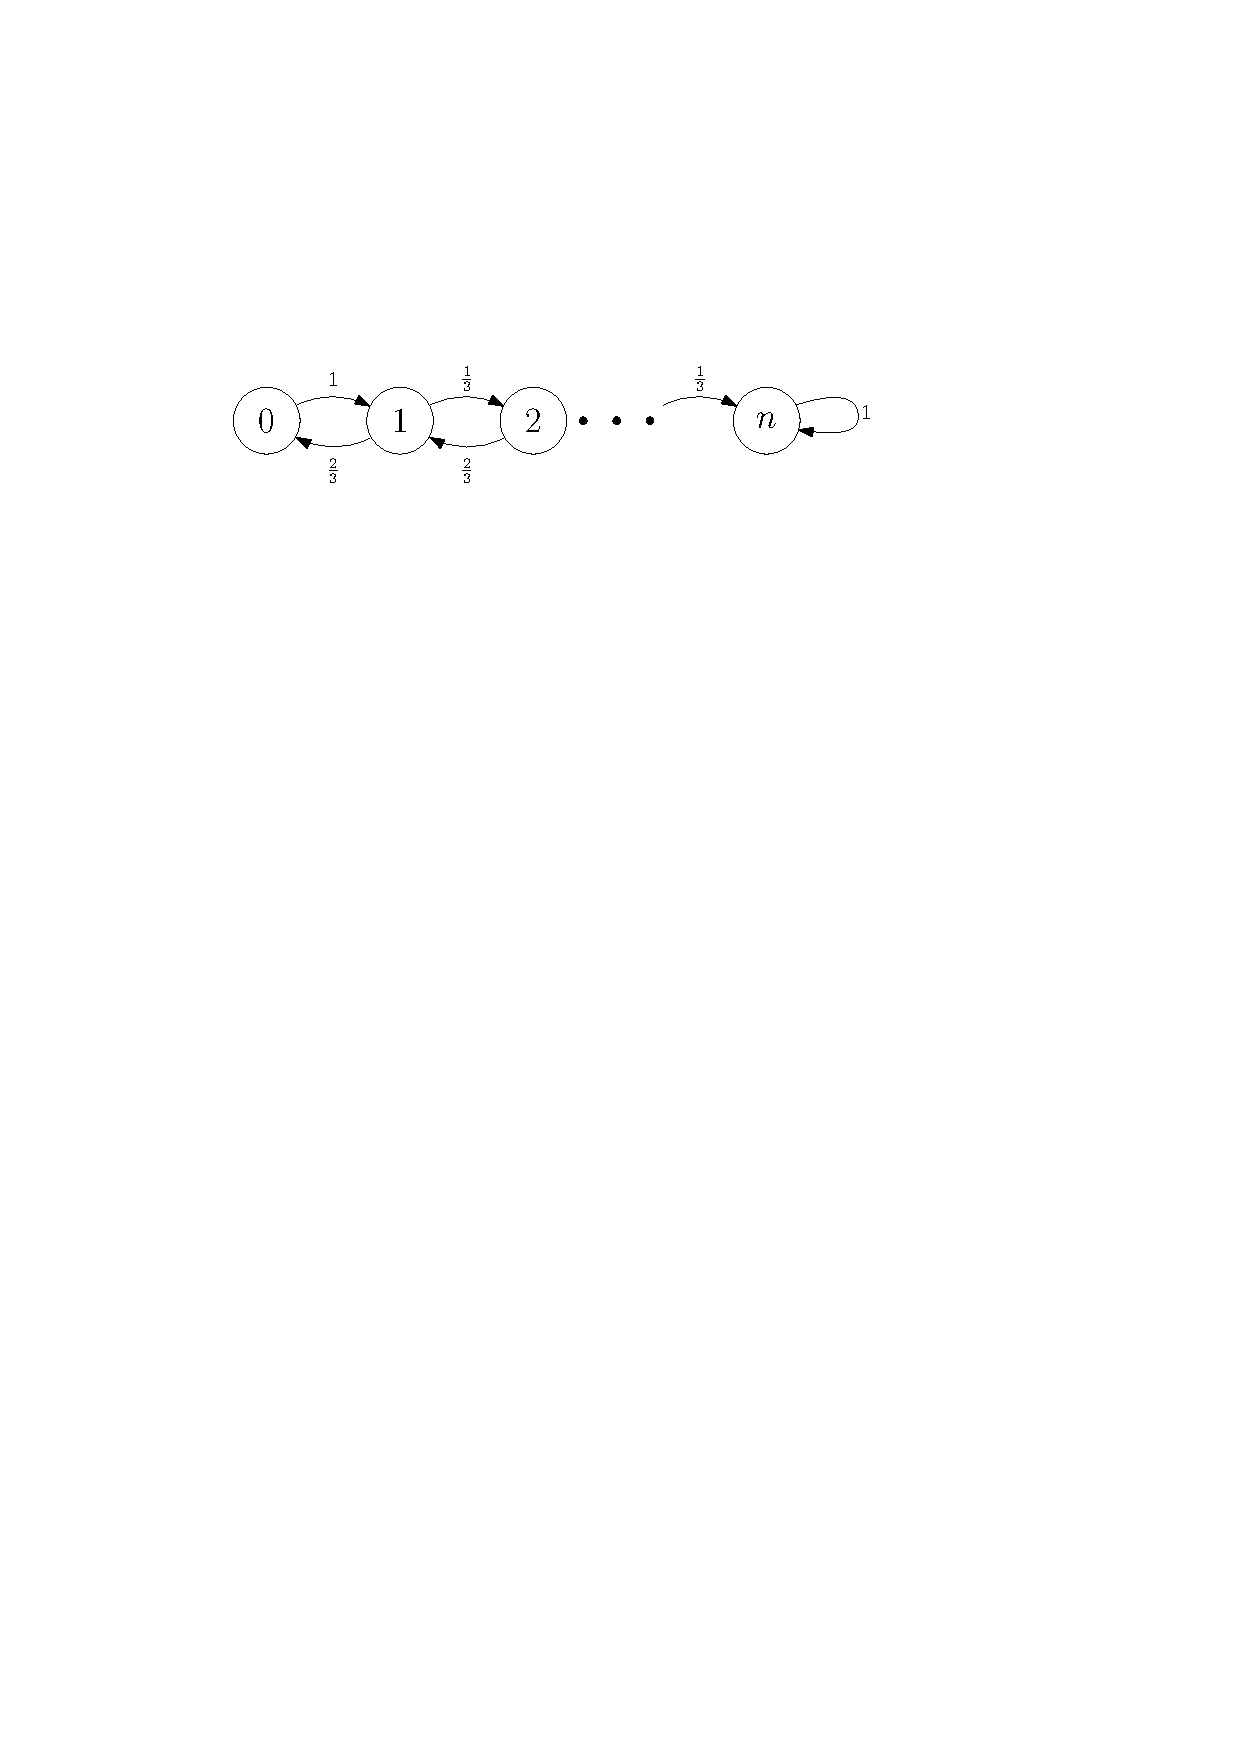
\includegraphics[width=0.5\linewidth]{markov-chain.pdf}
        \end{figure}

        Since Sch\"oning's algorithm uses a randomly assignment as the initial assignment, there is a $\binom{n}{u} / 2^n$ probability that the initial solution will be $u$ Hamming distance away from the satisfying assignment. So now suppose we are at a state $u$ steps away from the final state. We would like to find a lower bound on the probability of reaching state $n$ in at most $6n$ moves. Since $u \leq n$, this probability is lower bounded by the probability of reaching state $n$ in at most $6u$ steps. This is in turn lower bounded by the probability of moving $2.5u$ steps in the wrong direction and $2.5u + u$ in the right direction. This is a lower bound on the overall probability of succeeding because it is just one of many ways to reach $n$ within $6u$ steps.

        This gives us a lower bound of
        $$
        \sum_{u=0}^n \left[ \binom{n}{u} \cdot \frac{1}{2^n} \cdot \binom{6u}{2.5u} \cdot \left( \frac{1}{3} \right)^{3.5u} \cdot \left( \frac{2}{3} \right)^{2.5u} \right].
        $$
        We can bound the binomial coefficient using Stirling's approximation:
        $$
        \begin{aligned}
            \binom{6u}{2.5u} &= \frac{(6u)!}{(2.5u)! (3.5u)!} \\
            &\approx \frac{\sqrt{2\pi(6u)}}{\sqrt{2\pi(2.5u)} \sqrt{2\pi(3.5u)}} \cdot \left( \frac{6u}{e} \right)^{6u} \left( \frac{e}{2.5u} \right)^{2.5u} \left( \frac{e}{3.5u} \right)^{3.5u} \\
            &= \sqrt{\frac{12}{35\pi u}} \left( \frac{6^6}{2.5^{2.5} \cdot 3.5^{3.5}} \right)^u
        \end{aligned}
        $$
        so
        $$
        \binom{6u}{2.5u} \cdot \left( \frac{1}{3} \right)^{3.5u} \cdot \left( \frac{2}{3} \right)^{2.5u} \approx \sqrt{\frac{12}{35\pi u}} \cdot 0.4567^u
        $$
        Hence, using the combinatorial identity, we give a bound on the overall probability of succeeding:
        $$
        \sum_{u=0}^n \binom{n}{u} \frac{1}{2^n} \cdot \sqrt{\frac{12}{35\pi u}} \cdot 0.4567^u \geq \sqrt{\frac{12}{35\pi n}} \left(\frac{1+0.4567}{2}\right)^n \approx \sqrt{\frac{12}{35\pi u}} \cdot 0.72837^u
        $$
        which is slightly lower than the probability lower bound with $3n$ trials.
    \end{enumerate}
\end{enumerate}

\end{document}
